\documentclass[12pt]{article}
\usepackage{amsmath}
\usepackage{latexsym}
\usepackage{amsfonts}
\usepackage{amssymb}
\usepackage{graphicx}
\usepackage{txfonts}
\usepackage{wasysym}
\usepackage{adjustbox}
\usepackage{ragged2e}
\usepackage{tabularx}
\usepackage{hhline}
\usepackage{float}
\usepackage{multirow}
\usepackage{makecell}
\usepackage{fancyhdr}
\usepackage[utf8]{inputenc}
\usepackage[T1]{fontenc}
\usepackage[a4paper,bindingoffset=0.2in,headsep=0.5cm,left=1in,right=1in,bottom=3cm,top=2cm,headheight=2cm]{geometry}
\usepackage{hyperref}
\usepackage{listings}
\usepackage{color}

\definecolor{pblue}{rgb}{0.13,0.13,1}
\definecolor{pgreen}{rgb}{0,0.5,0}
\definecolor{pred}{rgb}{0.9,0,0}
\definecolor{pgrey}{rgb}{0.46,0.45,0.48}

\everymath{\displaystyle}
\pagestyle{fancy}
\fancyhf{}
\rfoot{Page \thepage}

\lstset{language=C,basicstyle=\footnotesize,keywordstyle=\color{red}\bfseries,  commentstyle=\color{blue}\textit,stringstyle=\color{green}\ttfamily, showspaces=false,showstringspaces=false}


\begin{document}
\sloppy 

\begin{center}
\Large Telecom Paris \\
\Large COMELEC Department \\
\vspace{20 pt}
\underline{\Huge Development Infrastructure for TTool}
\end{center}

\begin{table}[H]
\large
\centering
\begin{adjustbox}{width=\textwidth}
\begin{tabular}{ |p{1.6cm}|p{6.0cm}|p{4.4cm}|p{4.2cm}| }
\hhline{----}
 & \textbf{Document Manager} & \textbf{Contributors}  & \textbf{Checked by}  \\ 
\hhline{----}
\textbf{Name}   & Dominique BLOUIN & Ludovic APVRILLE &
\multirow{2}{*}{Ludovic APVRILLE} \\
\hhline{--~~}
\textbf{Contact} & dominique.blouin@telecom-paris.fr & \multirow{2}{*}{Arthur VUAGNIAUX} &  \\ 
\hhline{--~~}
\textbf{Date} & \today & Matteo BERTOLINO &  \\ 
\hline
\end{tabular}
\end{adjustbox}
\end{table}

\begin{figure}[!h]
\centering

\includegraphics[width=0.4\textwidth]{images/image1.png}
\end{figure}

\newpage
\tableofcontents

% \newpage
% \listoffigures

\newpage
\section{Preface}

\subsection{Table of Versions}

\begin{table}[H]
\large
\centering
\begin{adjustbox}{width=\textwidth}
\begin{tabular}{ |p{1.5cm}|p{2.5cm}|p{9.0cm}|p{3.0cm}| }
\hhline{----}
\textbf{Version} & \textbf{Date} & \textbf{Description  $  \&  $  Rationale of
Modifications} & \textbf{Sections Modified} \\
\hhline{----}
1.0 & 17/10/2016 & First draft &  \\ 
1.1 & 10/02/2017 & Added Eclipse IDE development + tests & All \\ 
1.2 & 11/02/2017 & Added more info on tests & Tests \\ 
1.3 & 02/10/2018 & Update and added GUI development & All\\
1.4 & 22/11/2018 & Added more info on automated tests and on the installer & Automated tests / Installer \\
1.4 & 11/06/2020 & Plugin: configuration, programming & Plugin \\
\hline
\end{tabular}
\end{adjustbox}
\end{table}

\subsection{Table of References and Applicable Documents}

\begin{table}[H]
\large
\centering
\begin{adjustbox}{width=\textwidth}
\begin{tabular}{ |p{2.66in}|p{2.66in}|p{0.95in}|p{0.43in}| }
\hhline{----}
\textbf{Reference} & \textbf{Title  $  \&  $  Edition} & \textbf{Author or
Editor} & \textbf{Year}
\\
\hhline{----}
 &  &  &  \\ 
\hline
\end{tabular}
\end{adjustbox}
\end{table}

\subsection{Acronyms and glossary}

\begin{table}[H]
\large
\centering
\begin{adjustbox}{width=\textwidth}
\begin{tabular}{ |p{1.24in}|p{5.45in}| }
\hhline{--}
\textbf{Term} & \textbf{Description} \\ 
\hhline{--}
 &  \\ 
\hline
\end{tabular}
\end{adjustbox}
\end{table}

\subsection{Executive Summary}

This document describes the development infrastructure that has been setup for
the development of TTool. It describes sources configuration management, the
development process with basic editor and command lines, with the Eclipse IDE,
as well as the testing, building and installation procedures.

\newpage 

\section{Source Configuration Management}
\label{sec:scm}

\subsection{Gitlab Server}

TTool sources are hosted on the Gitlab server of \textbf{Telecom Paris} under the
group \textbf{\textit{mbe}\textit{-tools}} and project \textbf{\textit{TTool}}. The Gitlab project
can be accessed via \url{https://gitlab.telecom-paris.fr/users/sign_in}. 
Login must be performed using Shibboleth as shown in
figure~\ref{fig:image1}, using the credentials from your institution if it is a
member of the Federation Education Recherche (\url{https://services.renater.fr/federation/participants/idp}). Otherwise, please ask us for an account.

\begin{figure}[H]
\begin{center}
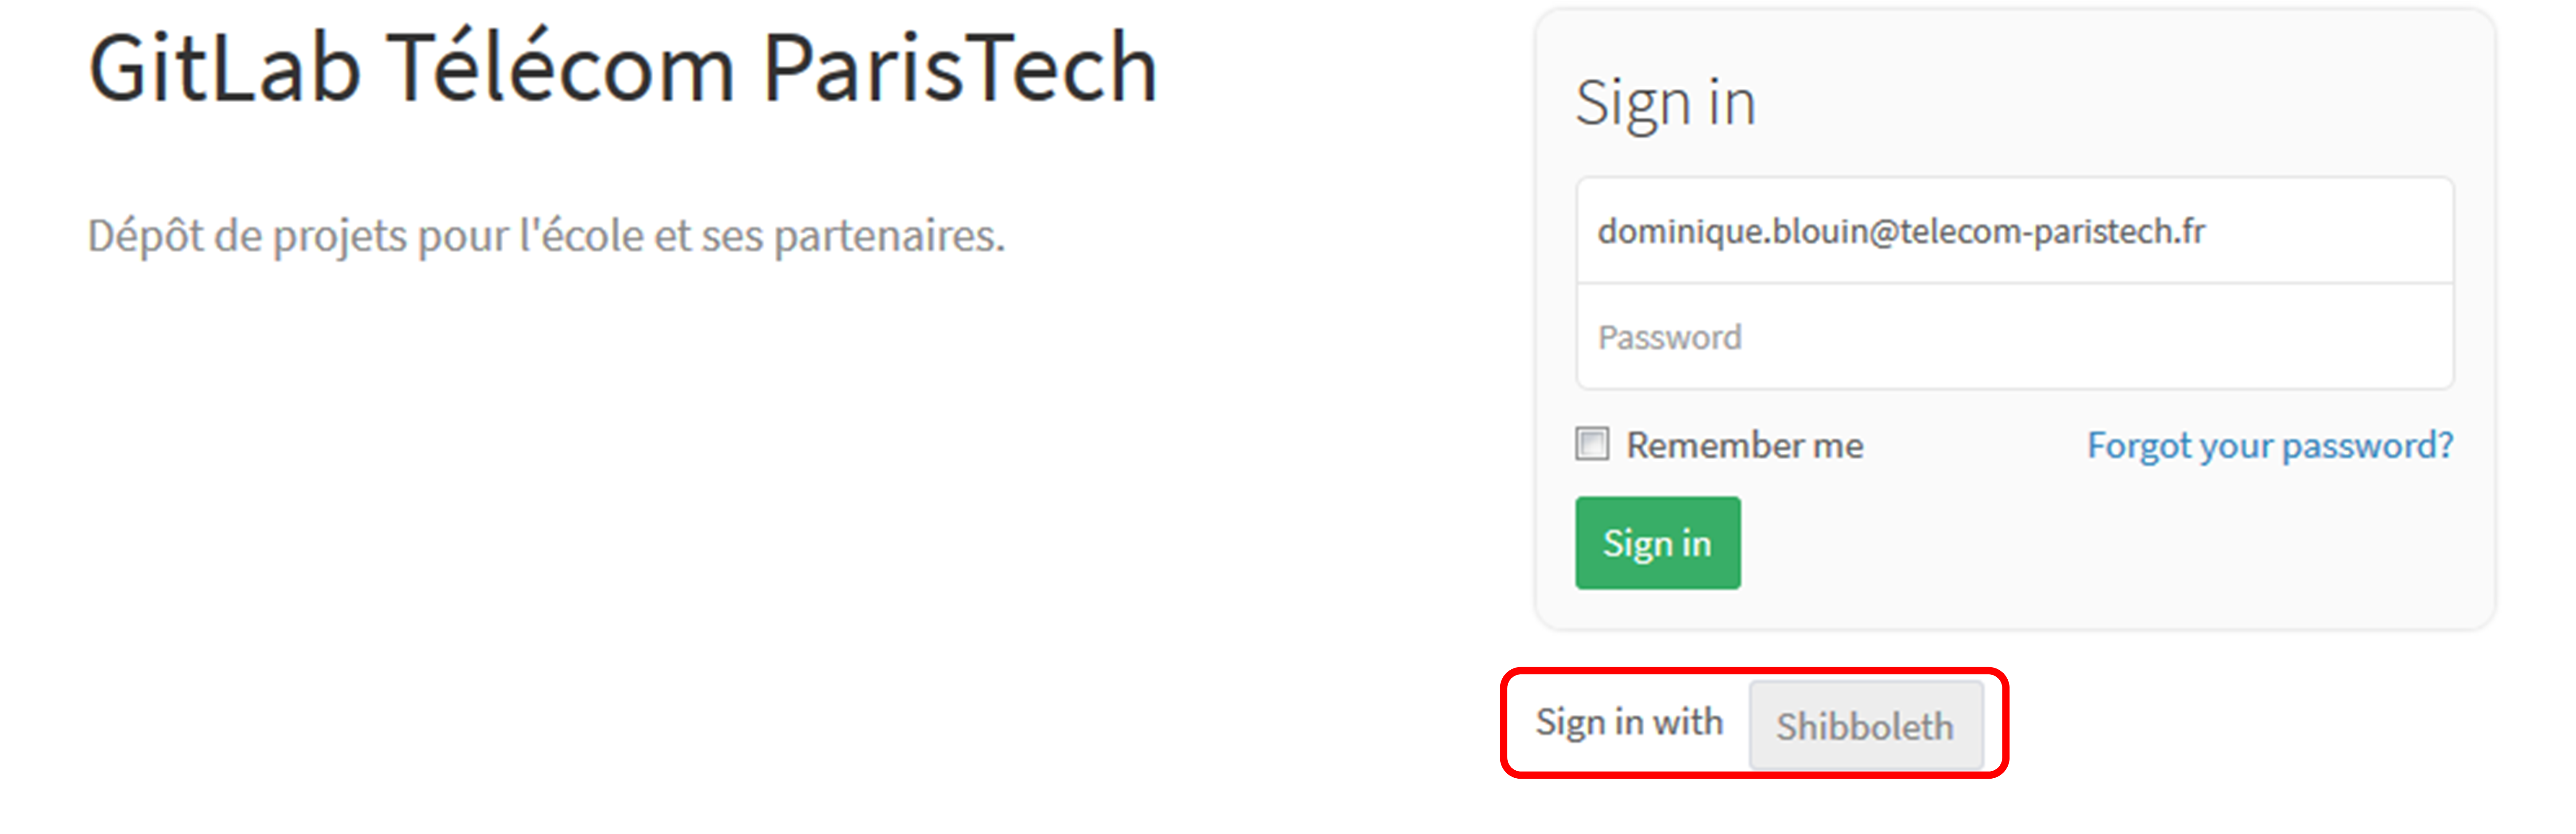
\includegraphics[width=\textwidth]{images/image2.png}
\end{center}
\caption{}
\label{fig:image1}
\end{figure}
 
\subsection{Basic Sources Management}

The address to access the sources is \url{https://gitlab.telecom-paris.fr/mbe-tools/TTool}.
For the time being and until further notice, we will keep using a centralized development process, like it was the case for Subversion. In this process, each developer first obtains a clone of the master remote repository. For this, go to the directory where the sources are to be downloaded and issue the following command: \\


\begin{verbatim}
git clone git@gitlab.enst.fr:mbe-tools/TTool.git
\end{verbatim}

Once modifications are made, they can be committed using command:

\begin{verbatim}
git commit -m "Commit message"
\end{verbatim}

This will only commit the changes in your local repository. In order to move them to the remote repository, use:

\begin{verbatim}
git push origin master
\end{verbatim}

More information on the use of Git can be found here: \\
\url{http://rogerdudler.github.io/git-guide/}. \\

By default, Git will ask credentials for each operation. In order to avoid this,
it is possible to upload a public SSH key at: \\
\url{https://gitlab.telecom-paris.fr/profile/keys}.

\subsection{Bug Tracking}

The Gitlab server provides an issues tracking system to record bugs, evolutions
or support demands from users and developers. Issues can be seen at: \\
\url{https://gitlab.telecom-paris.fr/mbe-tools/TTool/issues} \\

It is suggested to create an issue for every modification that is made to the
code, providing with the issue detailed information on the problem including
screen shots, log traces and test cases if required. This information is
important so that other developers can understand why the changes were made.
Ideally, the issue number should be mentioned within the modified code and
commit messages.  \\

\section{Development with Text Editor (emacs, vim) and Make}

The text editor of your choice can be used to edit the files of TTool. Yet, you must be sure that the correct indentation is respected. Use \textbf{4 spaces for each indentation level} and refer yourself to the \textbf{Coding Instruction} (\ref{sec:code_info}) .\\

Also, don't forget to insert your name at the top of the file in the authors list.\\

The main Makefile can be used to compile the source files of TTool, and to generate the jar libraries in bin/.
To compile TTool, do as follows, from the top directory of TTool:
\begin{verbatim}
42sh$ make ttool
\end{verbatim}

Other compilation targets can be obtained with:
\begin{verbatim}
42sh$ make help
\end{verbatim}
or:
\begin{verbatim}
42sh$ make
\end{verbatim}
In particular, compiling the sources of all subprojects can be done with the
\textit{all} target:
\begin{verbatim}
42sh$ make all
\end{verbatim}

\newpage

\section{Development with Eclipse}

Eclipse is a well-known Integrated Development Environment (IDE) providing many advanced functionalities to support developers and improve code quality by the application of built-in on the fly code analyses. One advantage of Eclipse is that it is a \textbf{multi-platform application} so it can be used on Linux, Windows and macOS. The procedures described in this section are valid for all platforms although some elements such as C++ projects need to be different due to different platform-specific compilation tool chains to be used. More information on this is provided on the concerned subsections.

\subsection{Installing and Configuring Eclipse}

Download Eclipse IDE for Java developers here: \\
\url{http://www.eclipse.org/downloads/packages/release/photon/r/eclipse-ide-java-developers}

Unzip the package and launch the eclipse executable. For developing C++
applications such as the DIPLODOCUS simulator, add the C Development Tools
(CDT). For this, select menu ``\textbf{Help >> Install New Software}''.
From the dialog box that opens, select the ``\textbf{Photon}'' update site, unfold the
``\textbf{Programming Languages}'' category and check the elements as shown in
figure~\ref{fig:image2}. Follow the wizard instructions to complete the
installation.

\begin{figure}[H]
\begin{center}
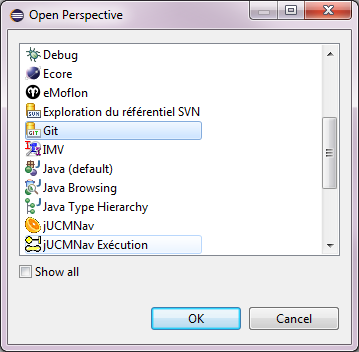
\includegraphics[width=0.9\textwidth, height=0.5\textheight]{images/image3.png}
\caption{}
\label{fig:image2}
\end{center}
\end{figure}

\subsection{Online Help}

The first place to look for help is in via menu ``\textbf{Help >> Help Content}'' from
Eclipse. A dialog box will show a tree with branches for each integrated plugin
or application. Help is provided for the 3 plugins that are used to develop
TTool; EGit, Java Development Tools and C/C++ Development Tools.

\subsection{Source Configuration Management with EGit}

The downloaded Eclipse IDE already includes a plugin named EGit for source
configuration management using Git.

\subsubsection{Cloning the TTool Repository}

First, switch to the Git perspective by clicking menu
``\textbf{Window >> Perspective >> Open Perspective >> Other}''. Then select the Git
perspective as illustrated in figure~\ref{fig:image3}.

\begin{figure}[H]
\begin{center}
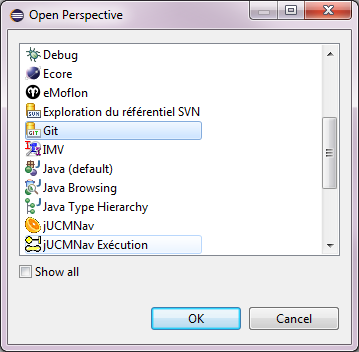
\includegraphics[width=0.6\textwidth]{images/image4.png}
\end{center}
\caption{}
\label{fig:image3}
\end{figure}

Then clone the TTool Git repository by clicking the appropriate button as shown
in figure~\ref{fig:image4}. Specify the \textbf{TTool Git repository URI}
(git@gitlab.enst.fr:mbe-tools/TTool.git) and follow the wizard by also setting
the local Git repository path.

\begin{figure}[H]
\begin{center}
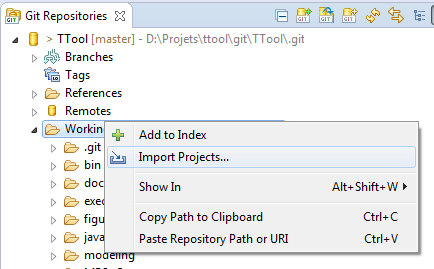
\includegraphics[width=0.6\textwidth]{images/image5.png}
\end{center}
\caption{}
\label{fig:image4}
\end{figure}

The content of the cloned repository can be seen from the Git Repository view by
unfolding the ``\textbf{Working Tree}'' folder (figure~\ref{fig:image5}).

\begin{figure}[H]
\begin{center}
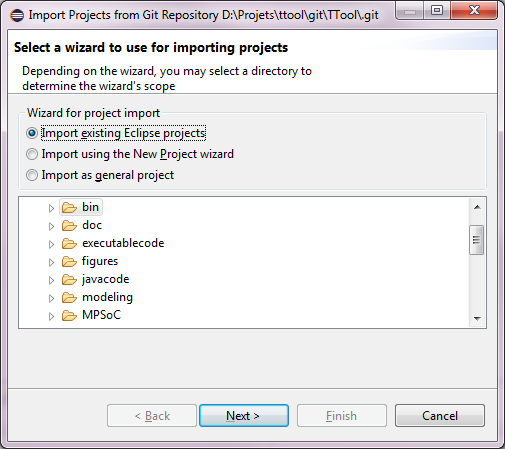
\includegraphics[width=0.6\textwidth]{images/image6.png}
\end{center}
\caption{}
\label{fig:image5}
\end{figure}

\subsubsection{Importing the Required Projects into the Workspace}
\label{sec:import}

Two Eclipse Java projects are needed to develop TTool: the \textit{bin} project
that contains the required libraries (jars) and the \textit{src} project that
contains the source code. Install these two projects in the workspace by
right-clicking the ``\textbf{Working Tree}'' it in the Git repository view and
selecting ``\textbf{Import Projects}\ldots'' as shown in figure~\ref{fig:image5}.

Then select ``\textbf{Import existing Eclipse projects}'' as shown in
figure~\ref{fig:image6} and follow the steps of the wizard.

\subsubsection{Committing, Pulling and Pushing Changes}

Committing the changes of a file or a directory or a project is performed by
selecting this element in the project navigator view then selecting
``\textbf{Team >> Commit}''. This will open the Git Staging view for where the changed
files are listed. Double clicking a file in the unstaged changes view will open
an editor allowing visualizing the changes (figure~\ref{fig:image7}). Right click and select
``\textbf{Add to Index}'', then enter a commit message and click the ''\textbf{Commit}'' button to
commit the changes. Pushing and pulling can be performed by selecting the repository from
the Git repository view or the elements from the project view.

\begin{figure}[H]
\begin{center}
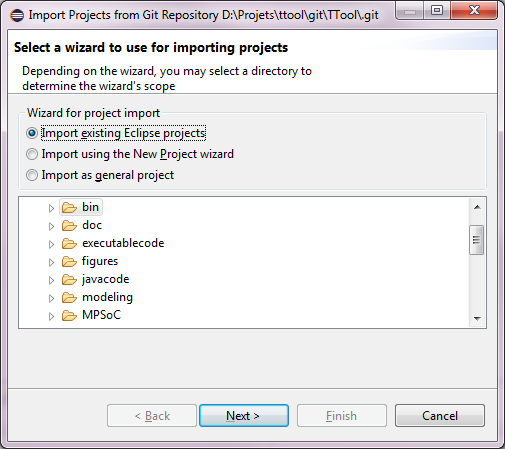
\includegraphics[width=0.6\textwidth]{images/image7.png}
\end{center}
\caption{}
\label{fig:image6}
\end{figure}

\begin{figure}[H]
\begin{center}
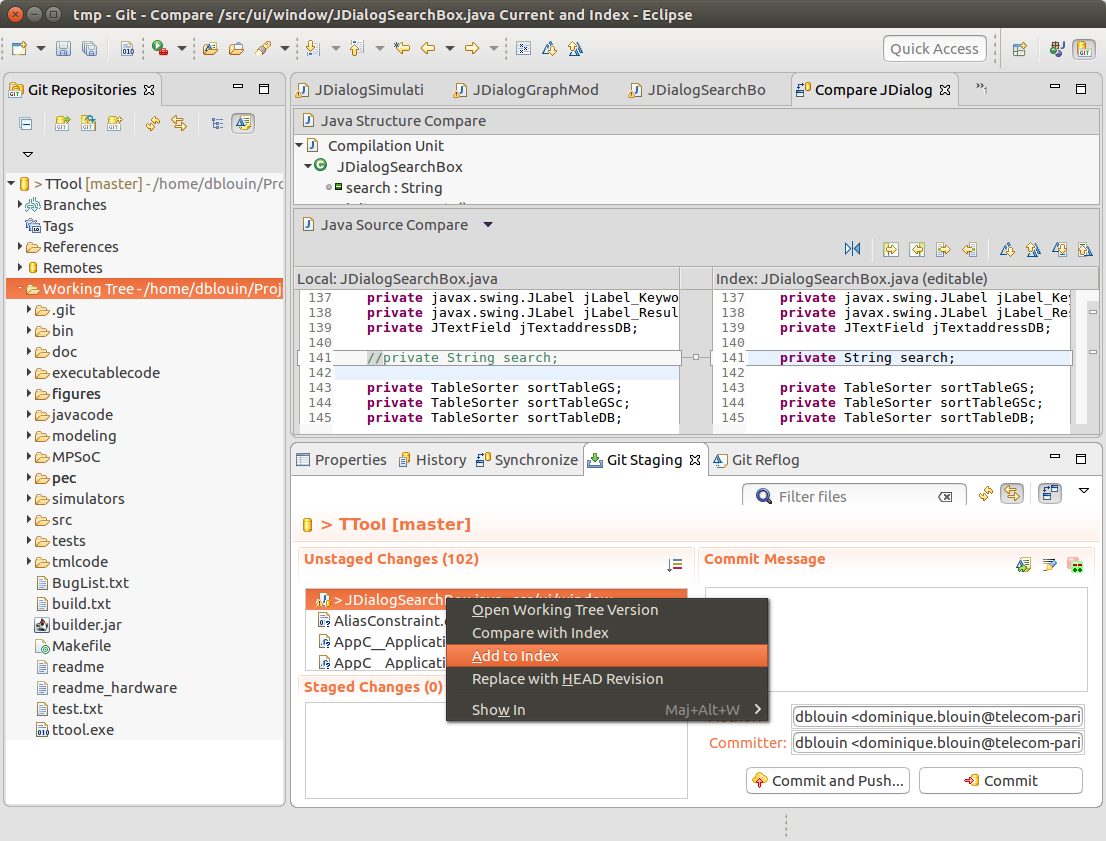
\includegraphics[width=\textwidth]{images/image8.png}
\end{center}
\caption{}
\label{fig:image7}
\end{figure}

\subsection{Java Development}

\subsubsection{Coding and Compiling}

Switch to the Java perspective to develop TTool with JDT (select menu
``\textbf{Windows >> Perspective}\ldots'' or select the appropriate perspective button from
the upper right corner of Eclipse). By default Eclipse will automatically
compile all files in the project. However the provided projects have already
been configured so that only the required classes are compiled and also to use
the required library files from the \textbf{\textit{bin}} project.

JDT provides several advanced functionalities such as automatically navigating
from a variable to its declaration, finding its use throughout all the classes,
including refactoring capabilities, syntactic coloration, code completion, etc.

\subsubsection{Launching TTool}
\label{sec:launch}

A default launch configuration is provided with the TTool \textbf{\textit{src}} project.
It allows for launching TTool from the compiled code. This configuration can be
edited by opening the \textbf{\textit{Run Configurations}} dialog box as show in figure~\ref{fig:image8}.

\begin{figure}[H]
\begin{center}
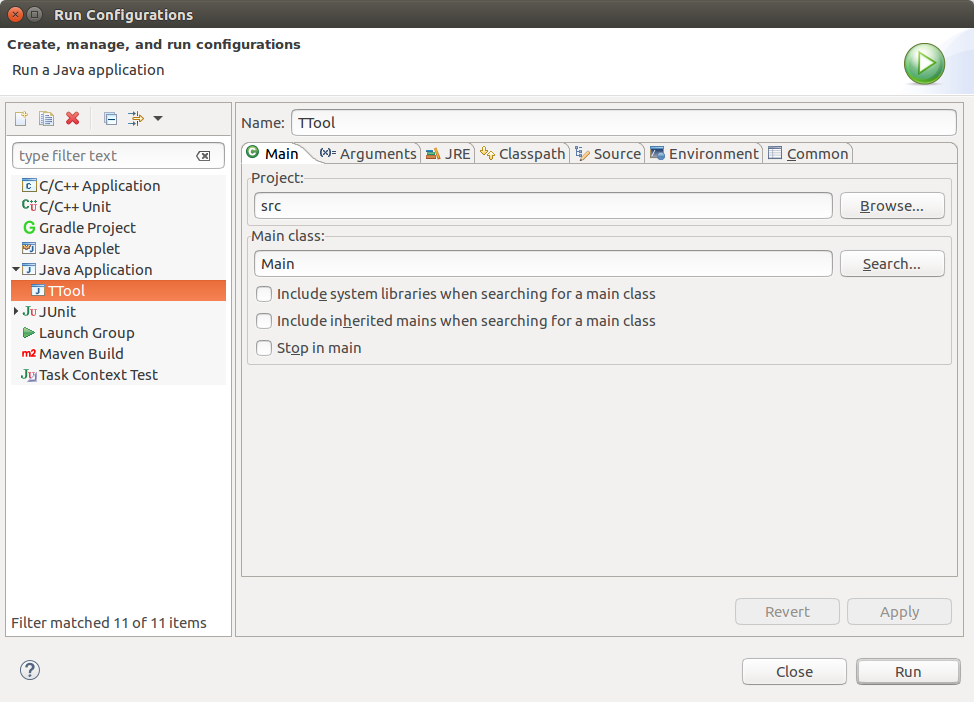
\includegraphics[width=0.9\textwidth]{images/image9.png}
\end{center}
\caption{}
\label{fig:image8}
\end{figure}

The TTool launch configuration is displayed in figure~\ref{fig:image9}. It
specifies the main class to execute as well as the program arguments, working directory and
optionally additional environment variables to be added to the default system
environment. Click \textbf{\textit{Run}} to launch TTool. The output from TTool will be
displayed in the console view. Once TTool has been launched once, simply
clicking the button to open the launch dialog box will directly launch TTool so
that it is not necessary to open the launch dialog box every time.

\begin{figure}[H]
\begin{center}
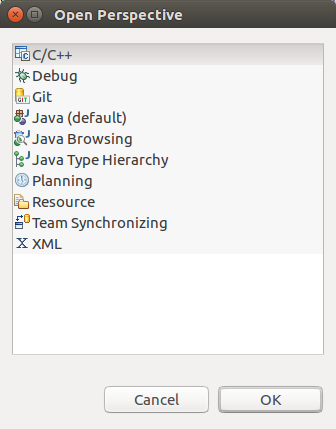
\includegraphics[width=\textwidth]{images/image10.png}
\end{center}
\caption{}
\label{fig:image9}
\end{figure}

\subsubsection{Using the Debugger}

In addition, JDT provides an enhanced debugger allowing executing the program
step by step with sophisticated breakpoints to control the execution and to
examine variable contents etc. However to use the debugger, the proper launch
configurations must be used by clicking the \textbf{\textit{debug}}
button just left of the launch configuration button of figure~\ref{fig:image8}.

\subsection{C++ Development}

One advantage of IDEs is that once a user has learned how to use a first tool,
other integrated tools are faster to learn because the tools share so much
functionality.

\subsubsection{Coding and Compiling}

Like for JDT, CDT also has its own perspective and the first thing to do is to
switch to this perspective as shown in figure~\ref{fig:image10}.

\begin{figure}[H]
\begin{center}
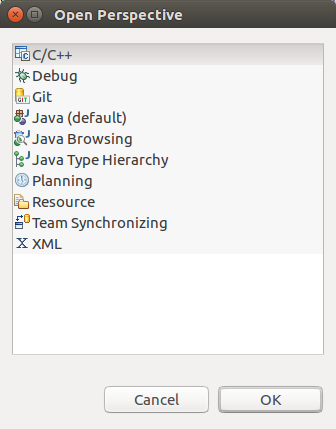
\includegraphics[width=0.45\textwidth]{images/image11.png}
\end{center}
\caption{}
\label{fig:image10}
\end{figure}

For developing the TTool C++ applications with CDT, the predefined CDT projects
must first be imported into the workspace as explained in
section~\ref{sec:import}. Note that for CDT, the projects are platform dependent
due to the different compilation toolchains (Cygwin is used for Windows) so there is one project per
platform. For instance, for developing the DIPLODOCUS simulator on Linux, import
the \textbf{\textit{c++2} project}. For windows, import the
\textbf{\textit{c++2 $  \_  $ windows} project} (TODO to be provided later). CDT
provides the ability to define several build configurations. For the
\textbf{\textit{c++2} project}, two configurations are provided as shown in
figure~\ref{fig:image11}.

\begin{figure}[H]
\begin{center}
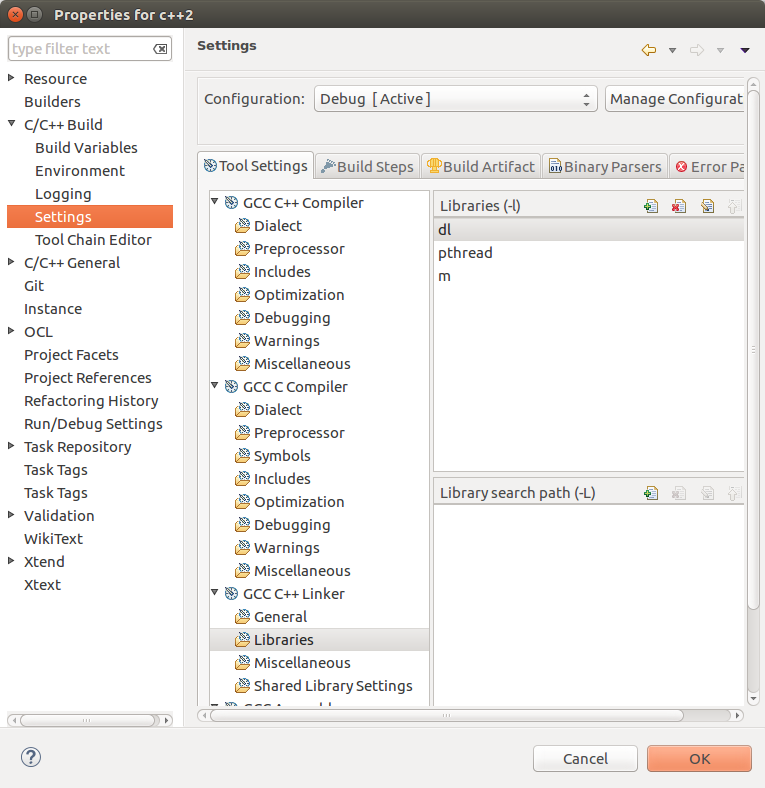
\includegraphics[width=0.9\textwidth, height=0.38\textheight]{images/image12.png}
\end{center}
\caption{}
\label{fig:image11}
\end{figure}

The \textbf{\textit{TTool} configuration} will compile the code using the provided make
file as if the simulator were compiled from TTool. The \textbf{\textit{Debug}
configuration} allows for compiling TTool such that it can be executed in debug
mode. The selected button in figure~\ref{fig:image11} allows changing the configuration being
used. The hammer button on the right hand side of it allows compiling and
linking the code.

The settings for these build configurations can be edited by selecting the
\textit{c++2} project in the project navigator and clicking
``\textbf{Properties}''. For the \textbf{\textit{Debug} configuration}, the CDT internal builder
is used. This means that the compilation and linking options can be changed via
the form editor shown in figure~\ref{fig:image12}.

\begin{figure}[H]
\begin{center}
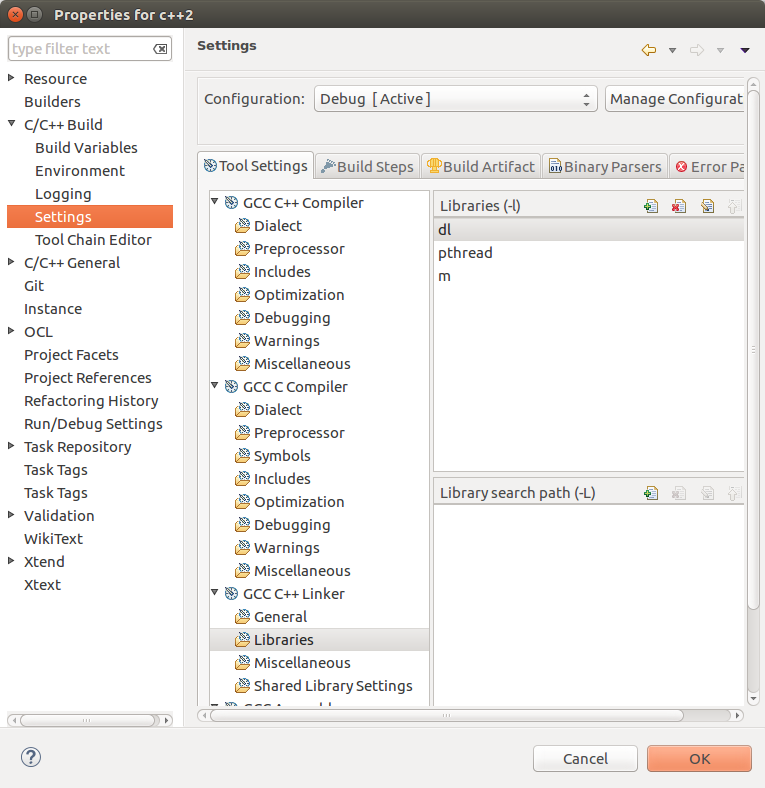
\includegraphics[width=0.9\textwidth]{images/image13.png}
\end{center}
\caption{}
\label{fig:image12}
\end{figure}

Note that the code provided by default in the \textbf{\textit{c++2} project}
from the Git repository does not compile by itself. TTool must first be executed
to generate the classes specific to the system being simulated. Once this is
done, the simulator can be compiled and executed from CDT for the desired build
configuration.

\subsubsection{Launching the Simulator}

Like for JDT, the launch of C++ applications can be specified using the launch
configurations dialog as introduced in section~\ref{sec:launch}. One launch
configuration is provided for each build configuration and named
\textbf{\textit{c++2 TTool}} and \textbf{\textit{c++2 Debug}}.

\subsubsection{Using the Debugger}

The CDT debugger is very similar to the JDT debugger. However to be able to use
it only the \textbf{\textit{c++2 Debug} launch configuration} should be used and
triggered from the \textbf{\textit{Debug As} button}. By default, the program execution
will automatically stop at the first instruction of the program. This behavior
can be changed by editing the debug launch configuration.

\newpage

\section{Development with IntelliJ}

IntelliJ IDEA is another Integrated Development Environment popular especially
among Java developers. It can be used to work on TTool and provides
functionalities globally similar to Eclipse.

\subsection{Installing and configuring IntelliJ}

Download IntelliJ IDEA here: \url{https://www.jetbrains.com/idea/}.

Unzip IntelliJ folder where you want to keep the executable. Launch it by using
the \textbf{\texttt{idea.sh}} script under the \textbf{\texttt{bin}} folder. Click on \textbf{\emph{Open}}
and navigate to the root of the TTool git repository.

\subsection{The IDE window layout}

A quick presentation of the user interface is given here:
\url{https://www.jetbrains.com/help/idea/guided-tour-around-the-user-interface.html}.
IntelliJ consists of an editor window and multiple tool windows. Some of the
important tool windows are:
\begin{itemize}
    \item \textbf{Project}. Show the structure of the project. In the case of
        TTool it displays the different sub-projects and the source folders
        (code, test, resource, etc.) for each sub-project. It can be used in
        addition to the navigation bar to navigate between files.
    \item \textbf{TODO}. List TODOs in the project files.
    \item \textbf{Structure}. Show the structure of a class (methods, fields,
        etc.).
    \item \textbf{Version control}. Show information related to the versioning
        system used (git in our case). This enables to see the commits that have
        modified the current file, the state of the various branches, the files
        that have been modified since the last commit or to directly make a
        commit.
    \item \textbf{Terminal}. This opens a pseudo-terminal window that can be
        used directly from IntelliJ.
\end{itemize}

Note that these tool windows are movable from the different panes and that the
toolbar that enables to select which tool window to display can be shown/hidden
by clicking on the icon on the lower-left side of the IntelliJ window.

\subsection{Debugging TTool}

IntelliJ integrates a debugger that is helpful to find some bugs. You can either
launch TTool in debug mode by clicking on the bug icon in the right part of the
navigation bar when the \textbf{\emph{TTool} configuration} is selected, or debug a
specific test by selecting \textbf{\emph{debug}} in the drop-down menu that appears when
clicking on the arrow for this test.

You can add breakpoints by clicking in the editor's left margin. You can the
right click on the breakpoint to modify it (log something, do not interrupt, add
a condition to the breakpoint, etc.). During debugging, when a breakpoint is
reached or the program was paused, you can see the current value of the
variables, see the stack frames, see the existing threads, add a watch point to
see how an expression evaluates, resume the program, execute step-by-step, etc.

\subsection{Configuring new sub-projects}
\label{sec:intellij:subprojects}

As described in section \ref{sec:code_orga}, TTool is composed of multiple
sub-projects. In IntelliJ, this is achieved by using \textbf{\emph{modules}}. You can see
the existing modules in the \textbf{\emph{File -> Project structure...}} menu. On the
left pane, click on \textbf{\emph{Modules}}. In particular, the \textbf{\texttt{shared} module }
consists of all the code used by other modules and the \textbf{\texttt{ttool} module} is
the main TTool application.

For each of these modules, you can add \textbf{\emph{content roots}} (path that will
contain sub-folders for sources, tests, resources and test resources). Then you
can select a sub-folder for a content root and mark it either as a source, test,
resource or test resource folder.

On the second tab, it is possible to modify the compile path. Note that if you
had a module then it must be compiled with gradle without requiring IntelliJ.
This is why you will need to update the compile path in order to generate the
output into the sub-project's build directory.

Finally, you can add dependencies in the third tab. This is useful in particular
if a sub-project requires an external library.

In the project structure window, on the left pane, you can select
\textbf{\emph{Artifacts}} to see the final results that can be built from the application
(the \texttt{ttool.jar} file for instance). As of today (February 2018), these
artifacts are:
\begin{itemize}
    \item some files needed by TTool during its execution
    \item the external libraries that TTool depends on
    \item the \texttt{ttool.jar} archive
\end{itemize}

\subsection{Configuration of code inspection and indentation rules}

IntelliJ enables to improve coding practice by providing warnings (e.g., unused
variable) that are
visible in the editor and by enabling to automatically correct them. These
warnings have different levels (error, warning, weak warning, etc.) and they are
fully configurable. In order to configure them, you can click on the icon at the
extreme right of the status bar and click on \textbf{\emph{configure inspections}}. You
can choose which inspection should be enabled and which warning level should be
raised when code does not follow these inspections. In order to provide a
common coding standard among TTool developers, the configuration of these
inspections is stored in a profile that is versioned by Git. You should thus not
modify this profile without asking other developers.

Similarly to these warnings, IntelliJ enables to harmonize code style by
defining a profile that is shared between all developers. To see the code style
options, go to \textbf{\emph{File -> Settings}} and navigate to
 \textbf{\emph{Editor -> CodeStyle}}. 
As for warnings, do not modify this shared profile except if you know
what you are doing.

Finally, IntelliJ enables to correct code style issues and some warnings
automatically. To do that, right click on the file in the project tool window
and select \emph{Reformat code}.

\subsection{Tips and tricks}

Note that there is a vim plugin available in IntelliJ that supports some of vim
commands.

\newpage 

\section{Coding Conventions}
Here are gathered all tricks on how TTool source codes are organized, and what function is coded where, and also how to extend TTool, e.g. adding a new diagram.

\subsection{Coding Instructions}
\label{sec:code_info}
\subsubsection{Best practices}

TTool is a constantly evolving project with more or less experimental parts. As
such, some leniency is expected from TTool developers and---while comments and
advice are always welcome---a perfect knowledge of best software engineering
practices should not be expected from every developers.

Nonetheless, we advise any developer to make her/his best to follow these best
practices. Indeed, the purpose of these principles is to enable the development
of easily understandable, extendable and reusable code. A good place to start if
you are not familiar with these principles is to have a look at the
\href{https://en.wikipedia.org/wiki/SOLID_(object-oriented_design)}{SOLID}
acronym.

In particular, developers should try to:
\begin{itemize}
    \item \textbf{Avoid public attributes}. Use getters and setters instead.
        This way, if the internal representation of the class changes, only the
        getters/setters would need to be modified.
    \item \textbf{Implement all of the methods of the superclass}.
        If some of the methods of the superclass are not relevant for the
        subclass, then it should probably not inherit from it. Indeed, other
        classes that uses the superclass logically assume that all of the
        subclasses implement the functionalities of the superclass.
    \item \textbf{Use abstractions instead of concrete
        classes when possible}. For instance, if an object A of package
        \textit{avatartranslator} must use an object B of package \textit{ui},
        create an interface in package \textit{avatartranslator} that is
        implemented by B and use it in A. This would make the low-level package
        \textit{ui} depend on the high-level package \textit{avatartranslator}
        instead of the opposite (which enables to use A in a CLI application for
        instance). This principle is also valid when the abstract class and its
        implementation are in the same package: for instance, prefer using
        \textit{List} objects in function arguments instead of the
        \textit{LinkedList} or \textit{ArrayList} concrete classes so that the
        caller can choose which subtype to instantiate.
\end{itemize}

\subsubsection{Style instructions}

\begin{itemize}
\item Indentations should use 4 spaces for each indentation level.
\item Opening brackets should be at the end of the line it relates to with one
    space before the bracket.
\item There should be 1 space between an \texttt{if}, \texttt{for},
    \texttt{switch}, etc. and the following opening parentheses, but none
        between a function name and the following parentheses.
\end{itemize}

Here is an example code with correct formatting : \\

\begin{lstlisting}[showspaces=true, language=java, commentstyle=\color{pgreen},
keywordstyle=\color{pblue}, stringstyle=\color{pred}, basicstyle=\ttfamily]
public class Foo {
    public int[] X = new int[]{1, 3, 5, 7, 9, 11};

    public void foo(boolean a, int x, int y, int z) {
        for (int i = 0; i < 5; i++) {
            try {
                if (x > 0) {
                    int someVariable = a ? x : y;
                    int anotherVariable = a ? x : y;
                } else {
                    for (int i = 0; i < 5; i++) doSomething(i);
                }
                switch (a) {
                    case 0:
                        doCase0();
                        break;
                    default:
                        doDefault();
                }
            } catch (Exception e) {
                processException(e.getMessage(), x + y, z, a);
            }
        }
    }
}
\end{lstlisting}

Do ensure your file is correctly indented before committing/pushing it.
Preferably, configure your code editor so that these guidelines are
automatically enforced. Also, for guidelines not given here, please apply the ones given in \href{https://google.github.io/styleguide/javaguide.html}{Java coding styles}.


\subsubsection{How to output debug information}
\label{sec:debug_info}
Do as follows:
\begin{lstlisting}
TraceManager.addDev("blah blah blah");
\end{lstlisting}
Then, start TTool with the 
\begin{verbatim}
 -debug
\end{verbatim}
option.
Thus, to print information, never use:
\begin{lstlisting}
System.out.println("blah blah blah");
\end{lstlisting}
or similar ways of doing.

\subsubsection{Warnings}
TTool is compiled with the following \textit{Xlint} warning flags:
\begin{itemize}
    \item unchecked
    \item deprecation
    \item cast
    \item divzero
    \item empty
    \item finally
    \item fallthrough
\end{itemize}
Before committing your changes, make sure that your code does not generate any
warning.

\subsubsection{Documentation}
Whenever it is possible, add a javadoc comment before any function, class or
field declaration. This helps future developers to quickly understand the
purpose of the related code. Note that to be valid, javadoc comments must be
placed right before the declaration and should be correctly formatted. To check
that it really is, generate the javadoc:
\begin{verbatim}
make documentation
\end{verbatim}
and make sure no warning is printed.

\subsection{Code organization}
\label{sec:code_orga}
The TTool repository actually hosts the source code of different standalone
projects. Here is a description of these sub-projects:
\begin{itemize}
    \item \textbf{ttool}. This is the main project: the TTool application with a
        graphical user interface.
    \item \textbf{graphminimize}. Command line application for minimizing graphs.
    \item \textbf{graphshow}. Command line application for displaying graphs.
    \item \textbf{launcher}. TODO 
    \item \textbf{rundse}. Application that run the \textbf{DSE} (\textit{Design Space Exploration}) of the current project. In \texttt{TTool/DIPLODOCUS}, the DSE evaluates the performance of a mapping solution by simulating the workload of computations and data-transfers
    \item \textbf{simulationcontrol}. Application that allow to simulate a remote control between an \texttt{host} and a \texttt{port}
    \item \textbf{tiftranslator}. This is the application for translating \textit{TIFT} to other languages (\texttt{LOTOS}, \texttt{RT-LOTOS}, \texttt{UPPAAL} or \texttt{JAVA}). The imput file should be in \textit{XML/TIF} format and be readable.
    \item \textbf{tmltranslator}. The application in order to tranlate \textit{TML} to other languages (\texttt{LOTOS}, \texttt{UPPAAL}, \texttt{SystemC}, \texttt{SystemC2} or \texttt{TML}). The imput file must be in \textit{TML} format and be readable
    \item \textbf{webcrawler}. Implement of a WebCrawler for \textbf{CVEs} (\textit{Common Vulnerabilities and Exposures}
        \begin{itemize}
            \item \textbf{client}. Client part of the WebCrawler 
            \item \textbf{server}. Server part of the WebCrawler
        \end{itemize}
    \item \textbf{jttool}. TODO \textit{(Development of this project has been
        dropped)}
\end{itemize}

For each of these sub-projects, there exists a folder in the TTool repository
that contains the sources, tests, resources and runtime dependencies associated
with it. Each of the sub-projects conforms to the
\href{https://maven.apache.org/guides/introduction/introduction-to-the-standard-directory-layout.html}
{Maven Directory Layout} and the root directory itself contains an \texttt{src}
folder which contains the source code shared by multiple sub-projects and
follow the same directory layout. This means that for instance, source code
specific to the \textit{ttool} sub-project should be located under
\texttt{ttool/src/main/java}, test classes related to the \textit{rundse}
sub-projects would be under \texttt{rundse/src/test/java} and resources (such as
images) needed by shared source code would be under \texttt{src/main/resources}.
Preferably, source code that would only be needed by a particular sub-project
should not be under \texttt{src/main/java} but under
\texttt{<project>/src/main/java}. In particular, \texttt{main} methods should
not appear in the shared source code directory (\texttt{src/main/java}).

If we focus on the shared sources, we see different packages. Basically, all
graphical-related elements are put in "ui". All other subdirectories of
\texttt{src/main/java}
are used to code generic functions (\texttt{myutil}") or non graphical languages and
model transformation. For example, in \texttt{avatartranslator/} you find all classes
related to the internal avatar language, and all transformations from the
internal avatar to other languages (e.g. to UPPAAL) are in subdirectories like
\texttt{avatartranslator/touppaal}. \textbf{Note}: please strive to provide
autonomous packages that depend on as few other packages as possible. This
enables to reuse code without including unrelated classes. In particular,
non-\texttt{ui} packages should not import \texttt{ui} classes so that a CLI
application that uses features provided by the package need not import the
graphical \texttt{ui} package.

\subsubsection{User Interface directories}
Main classes are located directly in "src/ui". Subdirectories of "ui/" are mostly used for diagrams (one diagram per subdirectory, e.g. avatarbd for the Avatar Block Diagram). Other subdirectories are explained in the following table.
\begin{tabular}{l|c}
subdirectory&Explanation\\
\hline
file&Contains the definition of file extensions used by TTool\\
graph&AUT graph definition, and how to display an AUT graph\\
interactivesimulation&Graphical part of Diplodocus model simulation\\
tree&tree located in the upper left part of the main TTool Window.\\
window&Sub-windows: dialogs, frames, etc.
\end{tabular}

\subsection{Structure of the User Interface}
Actions of the main user interface are defined in "TGUIActions.java". The corresponding method which is called when an action occurs is defined in "ActionPerformer.java".

\subsection{Structure of a diagram}


\subsection{Error management}
The tree on the left contains a part dedicated to errors and warnings. The list of errors/warnings that is displayed by the tree is handled in GTURTLEModeling.java with:
\begin{lstlisting}
private List<CheckingError> checkingErrors;
private List<CheckingError> warnings;
\end{lstlisting}

\newpage

\section{Testing}

It is planned to develop more and more tests for TTool in order to improve the
product quality. Test architectures are defined for each languages used to
develop TTool; Java and C++.

The testing code of TTool is located under the \textit{tests} directory of the TTool
repository and under \texttt{src/test/java} in any sub-project directory. A structure where a subdirectory is created for each
component of TTool to be tested (e.g.: Avatar, Diplodocus, shared utility
functions, etc.) is recommended. Each subdirectory can be further subdivided for
the different subcomponents of the component. For example, the Diplodocus component can be
further divided into its simulator and GUI components, which are not tested
under the same test environment and framework due to the different languages
used to develop these components.

A recommended practice consists of naming the folders containing the classes
with the same name of root package of the provided classes such as
$fr.tpt.ttool.tests.component\_name$, where $component\_name$ is the name of the
component of TTool being tested.

\subsection{Java}

The TTool Java code is tested using JUnit (\url{http://junit.org/}), which is a
unit test framework allowing to write, execute and display the results of
repeatable tests.

\subsubsection{Coding the Tests}

JUnit builds on a set of assertions for evaluating test results
and a set of annotations for qualifying test classes and methods. A test unit in
JUnit consists of a Java class grouping a set of test cases implemented as
methods of the class and identified with the $@Test$ annotation.
Other methods of the class to be executed only once before or after the
execution of all test cases of the class can be identified from the annotations
$@BeforeClass$ and $@AfterClass$. Methods to be executed before or after each
test case is executed can be identified from the annotations $@Before$ and
$@After$.

When using the Eclipse IDE, test classes can be automatically generated for a
given class to be tested and will include annotated methods for the selected
methods of the class to be tested.

With IntelliJ, when you are editing a Java class, you can jump to the corresponding test class
by right-clicking on the editor window (on a specific method or anywhere in the
class), and select \emph{Go To -> Test}.
IntelliJ will look for a corresponding test class and will propose to create a
new one. If you decide to create a new test class, select \emph{JUnit4} as the
testing library and pick the methods for which you want to add tests.

See folder $test/fr.tpt.ttool.tests.util$ of the TTool source code repository
for an example test class $TestRshClient$ providing test cases for the TTool
utility class $RshClient$ used for client-server remote communications.

\subsubsection{Executing the Tests}

\textbf{\emph{Using the JUnit Execution API}}

A JUnit test class can be executed automatically by passing
it to a JUnit test runner service that will take care of calling the appropriate
methods in the appropriate order to execute the tests, and return a test result
object that can be inspected to determine the success or failure of the test
cases and provide more details in case of failure. An example code snippet is
shown below:

\begin{verbatim}
import org.junit.runner.JUnitCore;
import org.junit.runner.Result;
import org.junit.runner.notification.Failure;
import fr.tpt.ttool.tests.util.remote.TestRshClient;

public class TToolUtilTestsRunner  {

    public static void main(String[] args) {
        Result result = JUnitCore.runClasses(TestRshClient.class);

        for ( final Failure failure: result.getFailures() ) { 
            System.err.println( "Test failed: " + failure.toString() );
        }
 		
        if ( result.wasSuccessful() ) {
            System.out.println( "All tests passed." );
        }
        else {
            System.err.println( "Some of the tests failed!" );
        }
 
        System.exit( 0 );
    }
}
\end{verbatim}

It is also possible to let gradle run the tests by invoking it:
\begin{verbatim}
gradle test
\end{verbatim}
or
\begin{verbatim}
gradle :ttool:test
\end{verbatim}
for a specific sub-project.\\

It, is also possible to run a given test, e.g.:
\begin{verbatim}
gradle :ttool:test -i --test cli.CLIAvatarModelCheckerTest
\end{verbatim}

A report is then generated under
\texttt{<project>/build/reports/tests/test/index.html}.

\textbf{\emph{Within the Eclipse IDE}}

Like for C++ and Java applications, JUnit launch configurations can be defined
in Eclipse as shown in figure~\ref{fig:image13}. This configuration will execute all unit tests
for class \textit{RSHClient} and display within the IDE a view of the status of
the tests (passed of failed) as shown in figure~\ref{fig:image14}.

\begin{figure}[H]
\begin{center}
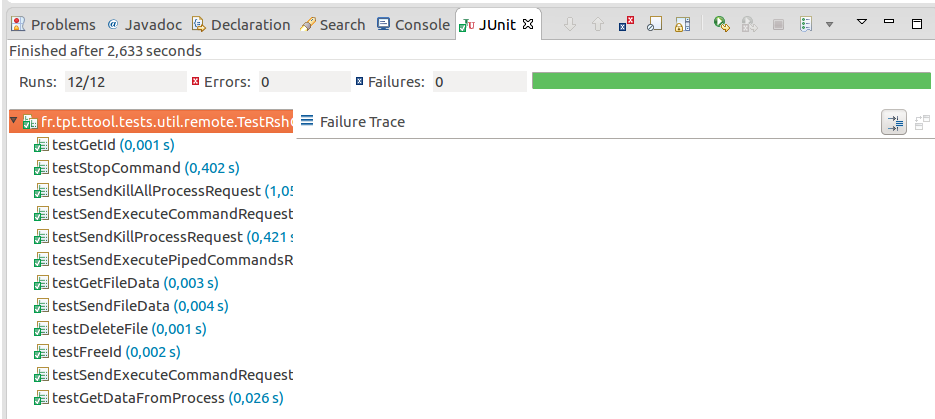
\includegraphics[width=\textwidth]{images/image14.png}
\end{center}
\caption{}
\label{fig:image13}
\end{figure}

\begin{figure}[H]
\begin{center}
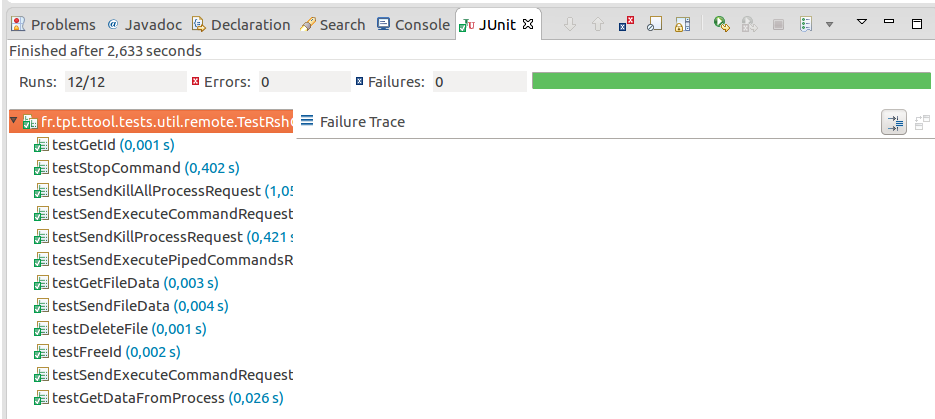
\includegraphics[width=\textwidth]{images/image15.png}
\end{center}
\caption{}
\label{fig:image14}
\end{figure}

\textbf{\emph{Within the IntelliJ IDE}}

Once the
test is written, you will have a green arrow in the left margin of the editor
next to each test method. You can either click on the arrow corresponding to a
specific method to run the corresponding test, or click on the arrow next to the
class name to run all the tests in this class.

In some cases, the tests need to use resources. You need to add these resources
to the \emph{test resources} root folder (see section
\ref{sec:intellij:subprojects} to see how this root folder is configured) and
to ensure that the test is running from the correct directory. To do this, run
the test once. You will see in the right section of the navigation bar a
shortcut to run the previous test. Expand the configuration selection list and
click on \emph{Edit Configurations...}. You can see all the available
configurations and modify options for each of them. In particular, you can
change the \emph{Working directory} (which should probably be
\texttt{ttool/build}) or require actions to do before running this
configuration (at the bottom of the window). You can share your configurations
so that other can use them but be careful not to share something with absolute
paths.


\subsection{C++}

TODO

\newpage

\section{Building}

\subsection{Compiling and Packaging}

First obtain the TTool repository from the Gitlab server as explained in section
\ref{sec:scm}. From a Linux shell, CD to the root TTool directory and execute
\emph{make all} to compile the code. If the compilation fails with the following error:
``unmappable character for encoding ASCII'', you need to do:

\emph{export JAVA\_TOOL\_OPTIONS=-Dfile.encoding=UTF8} \\

For generating a release, execute \emph{make release}.

\subsection{Gradle}
The TTool project has been configured so that it can be built with the
\href{https://gradle.org/}{Gradle Build Tool}. To this end, a
\texttt{build.gradle} file
is present in the root folder and each sub-project directory. Each
\texttt{build.gradle} file describes how to compile and package the related
sub-project and the \texttt{build.gradle} in the root folder describes shared
configuration. They should be modified when the compilation for a project
changes. In particular:
\begin{itemize}
    \item If a .jar library should be added to the classpath
    \item If a source folder should be added to the sourcepath
    \item If a javac flag should be added or removed
\end{itemize}

There is another gradle configuration file in the root folder of TTool:
\texttt{settings.gradle}. The purpose of this file is to list the sub-projects
of TTool. It should thus be modified when a new sub-project is created or if you
want a sub-project not to be compiled when calling \texttt{gradle build}.

In order to build all projects, run:
\begin{verbatim}
gradle build
\end{verbatim}
or 
\begin{verbatim}
gradle :ttool:build
\end{verbatim}
if you only want to build TTool.

\subsection{Executing TTool}
When TTool is executed, it fetches configuration settings from a
\texttt{config.xml} file and modifies it when closed. When you build TTool, a
default \texttt{config.xml} file is copied from
\texttt{ttool/runtime/config.xml} to \texttt{bin/config.xml}. As the
\texttt{bin} folder is not tracked by git, you can modify this configuration
file without committing your personal changes to the distant repository---which
you should not do. However, building TTool once again would replace your
personal \texttt{bin/config.xml} with the generic
\texttt{ttool/runtime/config.xml}, losing the changes you made on your
configuration file.

A better way to use your personal configuration file through different TTool
builds is to keep your own copy of \texttt{config.xml} outside of the
\texttt{bin} folder (which is removed when calling \texttt{make ultraclean}).
You can either create your own configuration file anywhere on the repository and
be careful not to add it to be tracked by git, or put it in a location where it
would not appear when doing a \texttt{git status}: either outside of the TTool
folder, or in a \texttt{.ttool} subdirectory which is explicitly ignored by git:
\begin{verbatim}
$ mkdir .ttool
$ cp ttool/runtime/config.xml .ttool/
\end{verbatim}
You could thus either call ttool directly:
\begin{verbatim}
$ java -jar bin/ttool.jar -config .ttool/config.xml
\end{verbatim}
or copy \texttt{ttool.exe} to \texttt{.ttool} subdirectory and modify it:
\begin{verbatim}
$ cat .ttool/ttool.exe
#!/bin/sh

java -version
cd .ttool;
java -Xmx1024m -Djavax.net.ssl.trustStore=ServerKeyStore \
    -Djavax.net.ssl.trustStorePassword=123456  -jar ../bin/ttool.jar \
    -config config.xml -experimental -debug -avatar -uppaal -launcher

$
\end{verbatim}

\newpage

% \section{GUI Automated Tests}
% \subsection{Research Stage}
% In order to find the right framework, it needed to put some criteria in our research to determine : \textit{What is a good GUI automated testing framework ?}
% After research, to answer this question, we need : \textit{"Flexibility, Capacity to work with the other framework already implemented and to be updatable"}
% But this criterias are not enougth to make a good and stable framework. \newline
% Then, for it, the team added the following criteria :
% 
% \begin{itemize}
%   \item \textbf{Work on all operating systems}: to work on MacOS, Linux and Windows
%   \item \textbf{Good Documentation}: to have a simple, understable documentation wioth possibly tutorials or others things
%   \item \textbf{Support Java}
%   \item \textbf{Support Swing}
%   \item \textbf{Open Source}: and possibly have a simple meaning to see the source
%   \item \textbf{Test Automation}: Unit test with a robot
%   \item \textbf{Regression Testing}: re-running functional/non-functional test to ensure that previously developed and tested software still performas
%   \item \textbf{Flexible}
%   \item \textbf{Record and Replay capabilities}: to record and replay the test
%   \item \textbf{Living Framework}: Updated regulary
%   \item \textbf{Work with other frameworks}
% \end{itemize}
% 
% After a few weeks of research, it had been decided to choose the framework named \textbf{AssertJ}
% 
% \subsection{AssertJ}
% AssertJ is a project developed by \textbf{Joel Costigliola}, which purpose is to rovides a fluent interface for writing assertions. 
% AssertJ is a fork of a previous project named \textbf{FEST Assert}. Its main goal is to improve test code readability and make maintenance of tests easier.
% AssertJ works like a Java Library and support also Swing.\newline
% In order to create the automated tests sequence, we use a part of the library, named \textbf{AssertJ Swing}.
% AssertJ Swing is based on JDK standard types assertions and can be used with either JUnit or TestNG. \newline
% The current verion of AssertJ Swing use in this project is the \textbf{3.8.0}, which works with \textit{Java 8} or higher.
% 
% \newpage
% 
% \subsection{Coding Instructions}
% Before doing any tests, make sure that all the libs are present and available. \newline
% If you are coding under an Integrated Development Environment (IDE) as Eclipse or IntelliJ, you should also download the AssertJ plugin. More informations here for :
% 
% \begin{itemize}
%    \item \textbf{Eclipse}: \url{http://joel-costigliola.github.io/assertj-eclipse-plugin/}
%    \item \textbf{IntelliJ}:\url{https://plugins.jetbrains.com/plugin/10345-assertions2assertj}
% \end{itemize}
% 
% All the files about this automated sequence of tests, are in the following directory : \textbf{ttool/src/test/java/ui/bot/}
% 
% \subsubsection{File Instructions}
% In order to create a class of tests, the developer need to find the package \textbf{ui.bot}, then to click on it and to select the tab \textbf{New/Class}.The developper will see the following window appear as in figure~\ref{fig:image15}:
% 
% \begin{figure}[H]
% \begin{center}
% 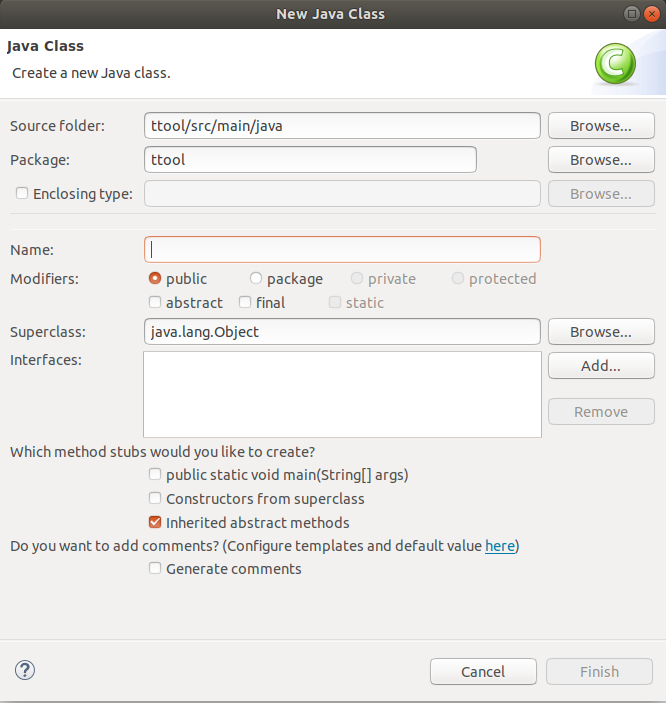
\includegraphics[width=0.8\textwidth]{images/image16.png}
% \end{center}
% \caption{}
% \label{fig:image15}
% \end{figure}
% 
% The developer only need to change one thing: the superclass of the class. The superclass has to be from \textbf{AssertJ library}, and the most useful one is the superclass \textbf{AssertJSwingJUnitTestCase} \newline
% The example in figuree~\ref{fig:image16} is what the developer should find as superclass.
% 
% \begin{figure}[H]
% \begin{center}
% 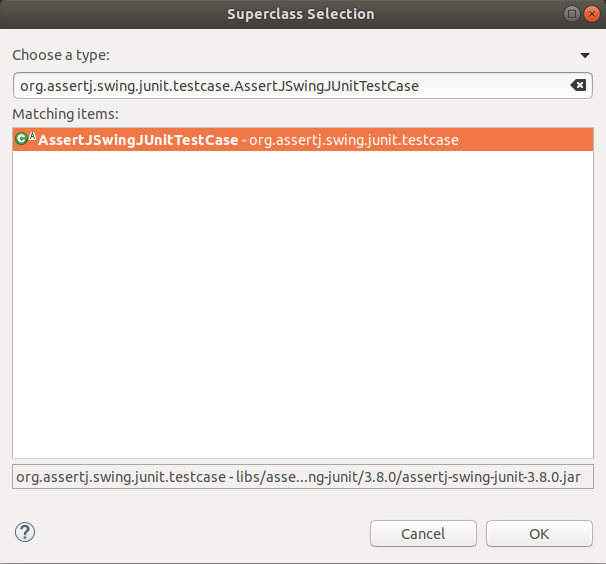
\includegraphics[width=0.9\textwidth]{images/image17.png}
% \end{center}
% \caption{}
% \label{fig:image16}
% \end{figure}
% 
% Now that constraint is done, here is the following files instructions:
% 
% \begin{itemize}
%   \item \textbf{Avoid bad names}: for the files, it has to be clear on what the developers are doing on the file itself.
%   \item \textbf{Not too much tests by files}: no more than 10 tests by files. Its avoid to have files with a lot of tests, to be lost between some tests, to have file with too much lines and also to have tests that have no record with the name of the file. Its allow the developer to find more quickly tests and to ensure the name of the file.
%   \item \textbf{Following the previous instructions}: see ~\ref{sec:code_info}
% \end{itemize}
% 
% The main function of each file will, if the developer do his job fine, have to extends \textbf{AssertJSwingJUnitTestCase}.Thus the developer will have to implement a method named : \textbf{onSetUp()} \newline
% This method has for purpose to initializes the test fixtures and to initializes also the frame on which tests are based. Here is an example of what could be the method :
% 
% \begin{verbatim}
% @Override
% protected void onSetUp() {
%    Main frame = GuiActionRunner.execute(()-> new Main(false, false, false, false, false, false, false, false, false, false, false, false, false));
%    window = new FrameFixture(robot(), frame.getFrame());
%    window.show();
% }
% \end{verbatim}
% 
% In this example there is some points to clarify. First of all the Main obeject is an object containing a frame (the frame on which the tests are based). The robot() in the definition of FrameFixture is not forced. The robot() allow to automate the test. Finally the window.show allow the user to see all the tests on the frame.\newline
% At the end of the file, it is better but not forced to have a method called \textbf{onTearDown()} whose aim is to clean up the frame fixture, thanks to the method named \textbf{cleanUp()}.
% Here is an example of the method onTearDown:
% 
% \begin{verbatim}
% @Override
% protected void onTearDown() {
%    super.onTearDown();
%    window.cleanUp();
% }
% \end{verbatim}
% 
% \subsubsection{Test Instructions}
% The following rules are:
% 
% \begin{itemize}
%   \item \textbf{@Test}: First of all, before eveything you need to precise that the method is a test. For that, the developer only need to put \textbf{@Test} before the name of the function
%   \item \textbf{Name}: Clear name in order to understand the meanning of the test
%   \item \textbf{Description}: Need to be clear and not too long on the subject of the test
%   \item \textbf{Trace in Console}: As saw in \ref{sec:debug_info}, the developer need to use TraceManager.addDev() to put some words in the console. Now the real utilisation of TraceManager here is to inform what the test is doing and to have a trace in the console. The fact that there is trace in the console allow to debug and to know where a test could fail.\newline
% The developer need to put a trace before and after an action is performed
%   \item \textbf{Debug}: For that the developer can usesome of the functions developed in the file UsefulTools.java. This file has some functions useful for debugging or even just transform a string into KeyEvent for an input
% \end{itemize}
% 
% With all the rules, here is an example of a fine test:
% \begin{verbatim}
% private FrameFixture window;
% private UsefulTools ut;
% private boolean debug = true;
% 
% @Test
% public void createANewFile() {
%    /*
%     * Description : Verify if TTool can create a new file, by clicking on the File menu then on
%     * the tab New. Then right click on it.
%     */
% 
%    TraceManager.addDev("==============" + System.lineSeparator() +
%                        "MainFrameTest: createANewFile: Started");
%    JMenuItemFixture jmf = window.menuItem("File New");
%    TraceManager.addDev("MainFrameTest: createANewFile: Creating a new file by clicking on New");
%    jmf.click();
%    if (debug)
%       ut.debugThread(3600, "MainFrameTest: createANewFile: ");
%    TraceManager.addDev("MainFrameTest: createANewFile: File created");
% 		
%    TraceManager.addDev("MainFrameTest: createANewFile: Right clicking on the file");
%    window.rightClick();
%    if (debug)
%       ut.debugThread(3600, "MainFrameTest: createANewFile: ");
%    TraceManager.addDev("MainFrameTest: createANewFile: Done clicking");
%    TraceManager.addDev("MainFrameTest: createANewFile: Finished" + 
%                        System.lineSeparator() + "==============");
% }
% \end{verbatim}
% 
% \subsubsection{Run as Configuration}
% 
% When you create a Configuration for a file of tests, in order to not have some bugs, you need to had some others files in the \textbf{Bootstrap Entries} \newline
% \begin{itemize}
% \item \textbf{AssertJ Swing}: you need to had all the assertj libraries for the swing (and of course the last version of them)
% \item \textbf{Ressources}: in \textbf{/src/main/}
% \item \textbf{src}
% \end{itemize}
% 
% As you can see in the following figure. Then you will need to save it. In order to save your configuration, you will need to go to the section \textbf{Common} and to save the configuration as \textbf{Shared file}
% 
% \begin{figure}[H]
% \begin{center}
% 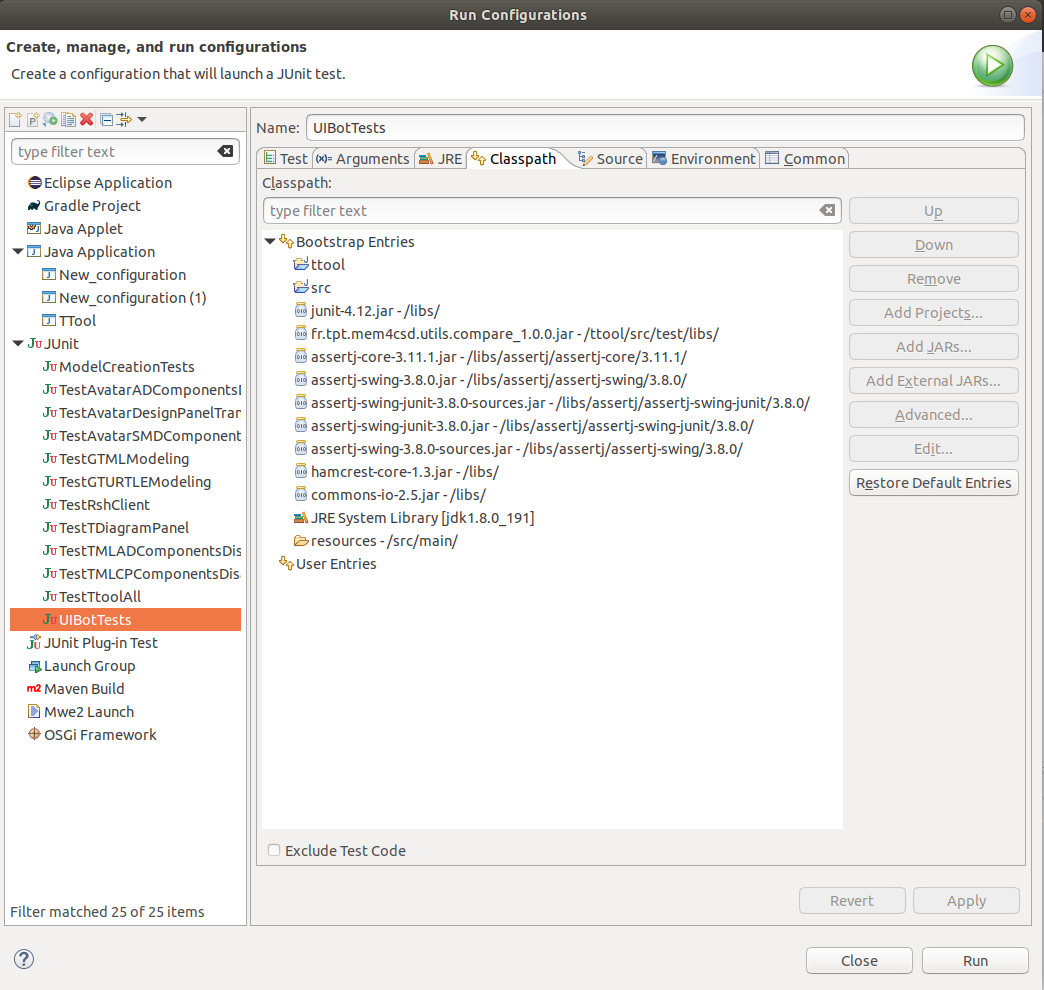
\includegraphics[width=0.9\textwidth]{images/image18.png}
% \end{center}
% \caption{}
% \label{fig:image17}
% \end{figure}
% 
% \newpage 

\section{TTool Installer}

This section documents the installer that was developed for TTool. The installer is using the IzPack tool for packaging Java applications.

\subsection{IzPack}

IzPack is an installer generator for the Java platform. It produces lightweight
installers that can be run on any operating system where a Java virtual machine
is available. Depending on the operating system, it can be launched by a
double-click or a simple 'java -jar installer.jar' on a shell. More information on IzPack can be found at:

\begin{itemize}
\item Main Page: \url{http://www.izforge.com/izpack/}
\item Documentation: \url{https://www.izforge.com/izpack/izpack-doc.pdf}
\end{itemize}

The current version of IzPack used by TTool is 5.1.3.

\subsection{Sources}

The sources of the installer are located in the TTool-Private Gitlab project at \url{https://gitlab.telecom-paris.fr/mbe-tools/TTool-Private/tree/master/installer}. 

\subsection{Configuration File}

The file \emph{install.xml} specifies the main configuration of the installer. The parameters are:

\begin{itemize}
	\item \textbf{info}: Section for project's informations.
	\item \textbf{guiprefs}: Graphical preferences (e.g.: size of window)
	\item \textbf{locale}: Set which language can be used in the installer
	\item \textbf{ressource}: All files used for by installer (html, images, etc.)
	\item \textbf{panels}: All panels used for the installer (in appearing order)
	\item \textbf{packs}: Sources of TTool, divided in packs
\end{itemize}

\subsection{Operating System Configuration}

There are some configuration files dependent on the operating system:

\begin{itemize}
	\item \textbf{Windows}: Named config\_win.xml
	\item \textbf{Linux}: Named config.xml
	\item \textbf{MacOs}: There is currently no configuration file for MacOs
\end{itemize}

\subsection{Companion Tools}

Besides installing TTool, the purpose of the installer is to install the many
companion tools of TTool such as \emph{Gtkwave} and \emph{Proverif}. The
binaries for those tools can be found under directory \emph{installer/lib}.

\subsection{Compilation of the Installer}

First, you have to export in an environment variable named \emph{JAVA\_HOME} the
path to your Java virtual machine directory (for example, /usr/lib/jvm/). The
script to compile the installer is \emph{src/compile.sh} passing the xml
configuration file of the installer as argument. In order to test the installer,
make a copy of the \emph{installer.xml} file and edit the paths to set the TTool
installation directory (IzPack does not allow to use a variable for this path).
However \textbf{do not push your changes ot the repository!} The install.xml is
configured for Ludovic Apvrille's computer and should stay as is for the
automatic build of the installer. In order to launch the installer, execute the
\emph{installer/src/install.exe} file from the \emph{installer/src} directory.

\section{Adding a Graphical Operator to a Diagram}
This section addresses the adding of a specific graphical component to a diagram. To better show how to do this, we use the example on how we have added a FPGA component to the DIPLODOCUS deployment diagram. A FPGA is a \textit{computation unit}, just like a CPU, but the steps listed are valid for any kind of graphical component like memories or communication nodes, of for any other diagram of TTool. A few things to remember:
\begin{itemize}
\item Add each new file (e.g. java file) that you create to the git repository, e.g.:
\begin{lstlisting}[showspaces=true, language=bash, commentstyle=\color{pgreen},
keywordstyle=\color{pblue}, stringstyle=\color{pred}, basicstyle=\ttfamily]
$git add myNewJavaFile
\end{lstlisting}
\item Remember also to change properly the \texttt{import} at the beginning of a java file if necessary. 
\end{itemize}
Adding a new component requires a serie of steps listed as follows: 

\paragraph{Deployment diagram:} The complete list of diagrams is located in \texttt{.src/ui} directory. In order to add a graphical component to the diagram we are interested in (e.g., \textit{TML Deployment Diagrams}), we first need to locate the corresponding sub-directory, in our case:  \texttt{tmldd}. Since our FPGA component is very similar to  the CPU component, we duplicated the class \textit{TMLArchiCPUNode.java} naming it \textit{TMLArchiFPGANode.java}. The main changes to do in this new class are: 
\begin{itemize}
\item \textbf{Stereotype}. Change the \texttt{String stereotype} value

\item \textbf{List of attributes}. Modify the list of attributes by adding or removing items: for example, we do not need the parameter \textit{number of cores} to describe the FPGA, so we removed \texttt{private int nbOfCores = HwCPU.DEFAULT\_NB\_OF\_CORES;}. Similarly, we need  a parameter that expresses the \textit{capacity} of the FPGA in terms of logical gates, so we added a new attribute.

\item \textbf{Manipulating attributes}. In order to manipulate the attributes, we weed to add/remove the corresponding setter/getter methods.
\texttt{private int capacity = HwCPU.DEFAULT\_CAPACITY;}

\item \textbf{Graphical connection and manipulation}. You can update graphic parameters such as: the connecting points (to connectors, including connectors for comments), the fact to make the diagrams editable, movable, removable, \ldots 

\item \textbf{Update the edition of the components' parameters}. Handle the lines like \texttt{if (dialog.getNbOfCores().length() != 0)} according with your previous modifications on the parameters' list. You can notice the usage of the \texttt{tmp} variable to recover the values in the case that the user closes the window or enters a non valid data (e.g., a word instead of a number).

\item \textbf{Unique identifier}. The method \texttt{public int getType()} returns a unique ID, defined in \texttt{TGComponentManager.java}. You thus need to update the two classes accordingly e.g., \texttt{public static final int TMLARCHI\_FPGANODE = 1116;} in \texttt{TGComponentManager.java} and  \texttt{public int getType()}. You have to choose an available number, and be sure to complete the switch/case in  \texttt{TGComponentManager.java}: one to create the component when the identifier is given, and one to obtain the identifier from a component:

In \texttt{TGComponentManager.java} you have also to add the new value that the \texttt{tgc} variable (that represents the graphical component) can take:
\begin{lstlisting}
 case TMLARCHI_FPGANODE:
                tgc = new TMLArchiFPGANode(x, y, tdp.getMinX(),
                      tdp.getMaxX(), tdp.getMinY(), tdp.getMaxY(),
                      false, null, tdp);
                break;
\end{lstlisting}

and 

\begin{lstlisting}
else if (tgc instanceof TMLArchiFPGANode) {
            return TMLARCHI_FPGANODE;
\end{lstlisting}



\item \textbf{Saving and loading the component}. TTool handles the saving and loading of default component attributes. Yet, for the specific attributes (e.g., the capacity of a FPGA), you need to explain to TTool how to save and load them. To save extra attributes, you can use the  \texttt{protected String translateExtraParam()} method e.g. add:
\texttt{sb.append("<attributes capacity=\"" + capacity + "\" byteDataSize=\"" + byteDataSize + "\" ");}

\item \textbf{Information on the component}. If the component implements the \texttt{WithAttributes} interface, then modify the \texttt{getAttribute()} method according to the new parameters. These methods are useful for the action \textit{Show/Hide element attributes} triggered by an icon in the architectural diagram, and for displaying an information in the status bar of TTool when the mouse is brought over the component.

\end{itemize}

\paragraph{Icon:} 
\begin{itemize}
\item Icons are stored in \texttt{./src/main/resources/ui/util}. You can easily use GIMP to create one of them, modifying an existing one to be sure to fit the proper dimensions. Don't forget to add the new icons to the git.

\item The class \texttt{.src/main/java/ui/util/IconManager.java} is responsible to load the icons when TTool starts. Let's assign a number to our icon. The convention is: an odd number for the \textit{big} sized icons, an even number for the \textit{small} sized icon. So, we assigned number 1120 to our new fpga icon: \texttt{private static String icon1120 = "tmlfpganode.gif";}

\item Next to the \texttt{//TDD} comment, create an object icon: \texttt{public static ImageIcon imgic1120;}

\item Associate the icon object to the previously defined string value: \texttt{imgic1120 = getIcon(icon1120);} 
\end{itemize}

\paragraph{Associate an action to the icon: } Actions list is contained in the file \texttt{.src/main/java/ui/TGUIAction.java}.
\begin{itemize}
\item The first step is to associate a unique number to the action that we aim to create. Let's search in the code for the parameter \texttt{public static final int NB\_ACTION = 474;}. All the actions are in a table named \texttt{private static final TAction [] actions = new TAction[NB\_ACTION];}. So, the number associated to our action should be equal to the number present in \texttt{NB\_ACTION}. Moreover, we need to reserve one more space for the action in the table, so we increment \texttt{NB\_ACTION} by one. In this case, \texttt{public static final int NB\_ACTION = 475;}.

\item Declare the action: taking inspiration from \texttt{public static final int TMLARCHI\_CPUNODE = 218;}, we similarly  create \texttt{public static final int TMLARCHI\_FPGANODE = 474;}

\item Then, add the action to the table, with the previously defined icon and a short description: 

\begin{lstlisting}
actions[TMLARCHI_FPGANODE] = new TAction("add-tmlarchi-fpganode", 
       "Add a FPGA node", IconManager.imgic1120, 
       IconManager.imgic1120, "FPGA node", "Add a fpga node to the 
       currently opened DIPLODOCUS architecture diagram", 0);
\end{lstlisting}

\item Finally, it is necessary to create the graphical component of such ID when this action on a FPGA node is triggered. To do that, open \texttt{.src/main/java/ui/ActionPerformer.java} and search for the string \texttt{CPUNode}. Then, similarly add:
 \begin{lstlisting}
else if (command.equals(mgui.actions[TGUIAction.TMLARCHI_FPGANODE]
		.getActionCommand())) {
            mgui.actionOnButton(TGComponentManager.COMPONENT, 
            TGComponentManager.TMLARCHI_FPGANODE);
\end{lstlisting}

\end{itemize}

\paragraph{Show and enable the icon in the diagram toolbar: }
\begin{itemize}
\item Open \texttt{.src/main/java/ui/tmldd/TMLArchiDiagramToolBar.java}
\item \textbf{Set the FPGA action as active} when the corresponding diagram is opened:
\begin{lstlisting}
protected void setActive(boolean b) {
     //[...]
     mgui.actions[TGUIAction.TMLARCHI_CPUNODE].setEnabled(b);
     mgui.actions[TGUIAction.TMLARCHI_FPGANODE].setEnabled(b);
     mgui.actions[TGUIAction.TMLARCHI_HWANODE].setEnabled(b);		
     //[...]
}		
\end{lstlisting}
\item\textbf{ Adding the FPGA icon to the toolbar}. 
Now, we are going to add the icon to the toolbar. 
Notice that the order is important! For example, we aim to place the FPGA icon before the HWACC icon and after the CPU node. Let's notice also that in order to add the icon we do not manipulate the icon object, but the action that contains the icon.
 
Since the implementation of the FPGA block was not still not supported by the DIPLODOCUS simulator when we created the graphical component, we hide the icon to regular users, and make it available only running TTool with the command line option \texttt{-experimental}. So, within the same class we can add the condition:
\begin{lstlisting}
if (mgui.isExperimentalOn()) {
            button = this.add(mgui.actions[TGUIAction.
                     TMLARCHI_FPGANODE]);
            button.addMouseListener(mgui.mouseHandler);
}
\end{lstlisting}
\end{itemize}

\paragraph{Dialog window:} Since the FPGA component is "editable", a double-click on it should open a dialog window in order to be able to edit the attribute of the corresponding component. The classes that handle the dialog box are usually located in \texttt{./src/main/java/ui/window}. Some complex components have these classes in their own subdirectories. 
\begin{itemize}
\item Let's have a look to \texttt{JDialogCPUNode.java}, copy/paste it, git add and modify the import.
\item Let's modify properly this new JDialog class. For example, we modified the JText fields and the getters in accordance to the declared parameters, we modified the constructor and we removed the stuff in which we're not interested on. The latter includes the things related to the MEC (useful for the code generation), tracemode, the useless grids, everything after the getters. 
\end{itemize}

\paragraph{Pivot language}.  TTool contains an internal pivot language that is used as an entry point to generate formal or textual specifications (e.g., C code). We therefore need to enhance the pivot language with the FPGA component.

\begin{itemize}
\item Let's have a look to \texttt{src/main/java/tmltranslator/HwCPU.java} and copy/paste it renaming the file \texttt{src/main/java/tmltranslator/HwFPGA.java} (don't forget to change the imports, and to add the new file to the git, as usual).

\item Modify the class according to your previous modifications. In particular, ensure the coherency between the list of attributes of your graphical component and of your pivot component. Then set their default value. Modify \texttt{toXML()} (useful for plugins) and \texttt{getType()} methods as well. 

\item Some attributes seems to be absent from the class  (e.g., \texttt{EXECI} and \texttt{EXECC}), but they are actually inherited from  \texttt{HwExecutionNode.java}, in the same package.

\item We also need to update the translation from the graphical DIPLODOCUs diagram to the pivot language. This translation is performed by the \texttt{.src/main/java/ui/GTMLModeling.java} class. In this class, we do quite exactly as for  \texttt{HwCPU cpu} and \texttt{TMLArchiCPUNode node}.
\end{itemize}


\paragraph{Textual representation (TML)} All the graphical components of DIPLODOCUS have a correspondence in  a textual format called TML. We thus need to add the FPGA component to the textual format as well, and to update the save and load functions to/from TML.

\begin{itemize}
\item Open \texttt{./tmltranslator/TMLArchiTextSpecification.java}.

\item Modify the string \texttt{private String keywords[] = {"NODE", "CPU", "FPGA", "SET", "BUS", "LINK", "BRIDGE", "MEMORY", "MASTERCLOCKFREQUENCY", "DMA"};} adding the FPGA word.

\item Exactly like for \texttt{private String cpuparameters[]}, declare \texttt{private String fpgaparameters[] = {"capacity", "byteDataSize", "mappingPenalty", "goIdleTime", "maxConsecutiveIdleCycles", "reconfigurationTime", "execiTime", "execcTime"};}. 

\item In the method \texttt{public String makeNodes(TMLArchitecture tmla)} let's declare \texttt{HwFPGA fpga;} variable, then have a look to \texttt{if (node instanceof HwCPU)} and handle similarly the corresponding FPGA case.

\item To load FPGA nodes from TML specification, consider the following method \texttt{public int analyseInstruction(String \_line, int \_lineNb, String[] \_split)}:
 \begin{lstlisting}
if (_split[1].equals("CPU")) {
                HwCPU cpu = new HwCPU(_split[2]);
                tmla.addHwNode(cpu);
            }
\end{lstlisting}
and do the same for the FPGA component.

\item Finally, in the same method, have a look to the case \texttt{if (node instanceof HwCPU)} and do the same for FPGA. To make the comparison easier, capitalize the name of the FPGA parameters. 
\end{itemize}   

\newpage
\section{Plugin}

A plugin makes it possible to add external features to TTool. 

\subsection{Installing a plugin}
A plugin is provided as a \textit{jar} file, for instance \textit{MyLovelyPlugin.jar}. For TTool to find and use this plugin, a configuration line must be added to the configuration file of TTool (e.g. \textit{config.xml}). For instance:

\begin{lstlisting}
<PLUGIN file="MyLovelyPlugin.jar" package = "mainstream"/>
\end{lstlisting}
means that the main class of the plugin, called "MyLovelyPlugin" shall be searched for in the "mainstream" package of the jar file. If the main class of the plugin is not in a package, then package must be left empty  \texttt{package=""}.


TTool searches for plugin in its default bin directory, or, if configured, in the \texttt{PLUGIN\_PATH}. Thus, the configuration file (e.g. \textit{config.xml}) can declare:
\begin{lstlisting}
<PLUGIN_PATH data="../plugins" />
\end{lstlisting}

\subsection{Programming a new plugin}

\end{document}
